\documentclass[10pt]{beamer}

\usepackage{amsmath,amssymb}
\usepackage{zxjatype}
\usepackage[ipa]{zxjafont}
\usetheme{metropolis}
\usepackage{tikz}
\usepackage{tikzsymbols}
\usepackage{appendixnumberbeamer}
\usepackage{bm}

\usefonttheme{professionalfonts}
\usetikzlibrary{positioning}

% -- block color ---
\setbeamercolor{block title}{use=structure, fg=white!90!purple, bg=purple!75!black}
\setbeamercolor{block body}{use=structure, fg=black!90!white, bg=white!90!black}
\setbeamercolor{block title example}{use=structure, fg=white!90!cyan, bg=cyan!75!black}
\setbeamercolor{block body example}{use=structure, fg=black!90!white, bg=white!90!black}

% --- page number ---
\setbeamertemplate{footline}{%
	\raisebox{10pt}{\makebox[\paperwidth]{\hfill\makebox[7em]{\normalsize\texttt{\insertframenumber/\inserttotalframenumber}}}}%
}

% --- title logo ---

\newcommand{\myinsertlogo}[1]{%
\begin{tikzpicture}[overlay, remember picture]
    \node[above left=1cm and .8cm of current page.south east] {\includegraphics[width=2.25cm]{#1}};
\end{tikzpicture}}

% --- commands ---

\newcommand{\redtext}[1]{\textcolor{red}{#1}}
\newcommand{\bluetext}[1]{\textcolor{blue}{#1}}
\newcommand{\highlight}[2][yellow]{\tikz[baseline=(x.base)]{\node[rectangle,rounded corners,fill=#1!10](x){$#2$};}}
\newcommand{\highlightcap}[3][yellow]{\tikz[baseline=(x.base)]{\node[rectangle,rounded corners,fill=#1!10](x){$#2$} node[below of=x, node distance=2em, color=#1]{#3};}}

\title{Probability Distributions (PRML \S2.3.1-2.3.7)}
\date{PRML Reading Club (June 3, 2019)}
\author{Satoshi Murashige}
\institute{Mathematical Informatics Lab., NAIST}

\begin{document}
    \begin{frame}[plain]
        \maketitle
        \myinsertlogo{naist.pdf}
    \end{frame}
    
    \begin{frame}{Table of Contents}
        \tableofcontents
    \end{frame}
    
    \begin{frame}{Review: Multivariate Gaussian Distribution}
        Hello metropolis!
    \end{frame}
    
    \section{\S2.3.1 Conditional Gaussian Distribution}
    
    \begin{frame}{Conditional Gaussian Distribution}
        Now, we consider to derive the following properties
        \begin{block}{Properties of conditional Gaussian distribution}
            \begin{align*}
                &p(\mathbf x_a, \mathbf x_b) = p(\mathbf x) = \mathcal N(\mathbf x | \bm \mu, \bm \Sigma) 
                \Rightarrow 
                \begin{array}{l}
                     p(\mathbf x_a | \mathbf x_b) = \mathcal N(\mathbf x_a | \bm \mu_{a|b}, \bm \Sigma_{a|b})  \\
                     p(\mathbf x_a) = \mathcal N(\mathbf x_a | \bm \mu_a, \bm \Sigma_a) 
                \end{array}
            \end{align*}
        \end{block}
        \begin{center}
            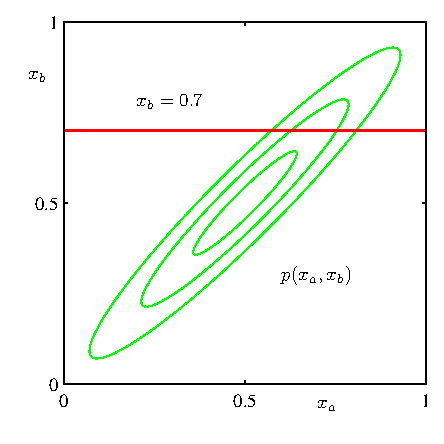
\includegraphics[width=0.45\hsize]{figs/Figure2_9a.pdf}
            \hfill
            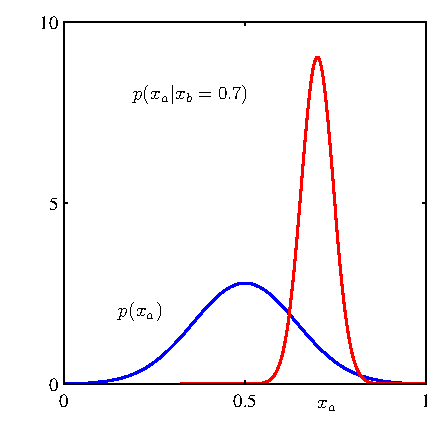
\includegraphics[width=0.45\hsize]{figs/Figure2_9b.pdf}
        \end{center}
    \end{frame}
    
    \begin{frame}{Examples of $\mathbf x_a$ and $\mathbf x_b$}
        \begin{exampleblock}{Sequence of a rocket's position}
            \begin{align*}
                &\mathbf x_a = x_{t+1} \\
                &\mathbf x_b = (x_1, x_2, \cdots, x_t)^\top
            \end{align*}
        \end{exampleblock}
    \end{frame}
    
    \begin{frame}{Definition of Notation}
        Consider a joint distribution $p(\mathbf x) = \mathcal N(\mathbf x | \bm \mu, \bm \Sigma)$
        \begin{itemize}
            \item Separate a $D$-dimensional vector $\mathbf x \sim \mathcal N(\mathbf x | \bm \mu, \bm \Sigma)$
                into $\mathbf x_a \in \mathbb R^M$ and $\mathbf x_b \in \mathbb R^{D-M}$
                \begin{align*}
                    \mathbf x &= \begin{pmatrix}
                        \mathbf x_a \\
                        \mathbf x_b 
                    \end{pmatrix} \tag{2.65}\\
                    \bm \mu &= \begin{pmatrix}
                        \bm \mu_a \\
                        \bm \mu_b 
                    \end{pmatrix} \tag{2.66}\\
                    \bm \Sigma &= \begin{pmatrix}
                        \bm \Sigma_{aa} & \bm \Sigma_{ab} \\
                        \bm \Sigma_{ba} & \bm \Sigma_{bb} 
                    \end{pmatrix} \tag{2.67}\\
                \end{align*}
        \end{itemize}
    \end{frame}
    
    \begin{frame}{Derivation of Conditional Gaussian Distribution}
    
    \end{frame}
    
    \begin{frame}{Title}
        \begin{block}{Closed form of conditional Gaussian distribution (still using $\bm\Lambda_{**}$)}
            \begin{align*}
                 &p(\mathbf x_a | \mathbf x_b) = \mathcal N(\mathbf x_a | \bm \mu_{a|b}, \bm \Sigma_{a|b})  \\
                 &
                 \begin{cases}
                 \bm\Sigma_{a|b} = \bm\Lambda_{aa}^{-1} \\
                 \bm\mu_{a|b} = \bm\mu_a - \bm\Lambda_{aa}^{-1}\bm\Lambda_{ab}(\mathbf x_a - \bm\mu_b)
                 \end{cases}
            \end{align*}
        \end{block}
        \begin{itemize}
            \item Where, we don't know a form of $\bm\Lambda_{aa}$ and $\bm\Lambda_{ab}$
        \end{itemize}
    \end{frame}
    
    \begin{frame}{Derivation of closed form of $\bm\Lambda_{**}$}
        \begin{block}{Exercise 2.24}
            \begin{align*}
                \begin{pmatrix}
                    \mathbf A & \mathbf B \\
                    \mathbf C & \mathbf D
                \end{pmatrix}^{-1} &= 
                \begin{pmatrix}
                    \mathbf M & -\mathbf M\mathbf B\mathbf D^{-1} \\
                    -\mathbf D^{-1}\mathbf C\mathbf M & \mathbf D^{-1}+\mathbf D^{-1}\mathbf C\mathbf M \mathbf B \mathbf D^{-1}
                \end{pmatrix} \tag{2.76}\\
                \mathbf M &= (\mathbf A - \mathbf B\mathbf D^{-1}\mathbf C)^{-1} \tag{2.77}
            \end{align*}
        \end{block}
        \begin{itemize}
            \item By applying above equations to
            \[
                \begin{pmatrix}
                    \bm \Sigma_{aa} & \bm \Sigma_{ab} \\
                    \bm \Sigma_{ba} & \bm \Sigma_{bb} 
                \end{pmatrix}^{-1}
                =
                \begin{pmatrix}
                    \bm \Lambda_{aa} & \bm \Lambda_{ab} \\
                    \bm \Lambda_{ba} & \bm \Lambda_{bb} 
                \end{pmatrix}, \tag{2.78}
            \]
            \item we cant get
            \begin{align*}
            \end{align*}
        \end{itemize}
    \end{frame}
    
    \begin{frame}{Title}
        \begin{block}{Closed form of conditional Gaussian distribution}
            \begin{align*}
                &p(\mathbf x_a | \mathbf x_b) = \mathcal N(\mathbf x_a | \bm \mu_{a|b}, \bm \Sigma_{a|b})  \\
                &\bm\mu_{a|b} = \bm\mu_a - \bm\Sigma_{ab}\bm\Sigma_{bb}^{-1}(\mathbf x_b - \bm\mu_b) \tag{2.81}\\
                &\bm\Sigma_{a|b} = \bm\Sigma_{aa}-\bm\Sigma_{ab}\bm\Sigma_{bb}^{-1}\bm\Sigma_{ba} \tag{2.82}
            \end{align*}
        \end{block}
    \end{frame}
    
    \begin{frame}{Derivation of Marginal Gaussian Distribution}
        \begin{align*}
            p(\mathbf x_a) &= \int p(\mathbf x_a, \mathbf x_b) \:\mathrm d\mathbf x_b \tag{2.83}\\
            &= \int \frac{1}{(2\pi)^{D/2}|\bm\Sigma|^{1/2}}\exp\left\{ -\frac{1}{2}(\mathbf x - \bm\mu)^\top \bm\Sigma^{-1}(\mathbf x - \bm\mu) \right\} \:\mathrm d\mathbf x_b \\
            &= \int \mathrm{const.} \cdot \exp(\redtext{\mbox{The terms involving $\mathbf x_b$}}) \cdot \exp(\bluetext{\mbox{Other terms}}) \:\mathrm d\mathbf x_b \\
            &= \mathrm{const.}\cdot \exp(\bluetext{\mbox{Other terms}}) \int \exp(\redtext{\mbox{The terms involving $\mathbf x_b$}}) \:\mathrm d\mathbf x_b
        \end{align*}
    \end{frame}
    
    \begin{frame}{Derivation of Marginal Gaussian Distribution}
        \begin{align*}
            &-\frac{1}{2}(\mathbf x - \bm\mu)^\top \bm\Sigma^{-1}(\mathbf x - \bm\mu) \\
            &=-\frac{1}{2}(\mathbf x_a - \bm\mu_a)^\top \bm\Lambda_{aa}(\mathbf x_a - \bm\mu_a)
            -\frac{1}{2}(\mathbf x_a - \bm\mu_a)^\top \bm\Lambda_{ab}(\mathbf x_b - \bm\mu_b) \\
            &\qquad -\frac{1}{2}(\mathbf x_b - \bm\mu_b)^\top \bm\Lambda_{ba}(\mathbf x_a - \bm\mu_a)
            -\frac{1}{2}(\mathbf x_b - \bm\mu_b)^\top \bm\Lambda_{bb}(\mathbf x_b - \bm\mu_b) \tag{2.70} \\
            %---------------
            &= -\frac{1}{2}\left( \mathbf x_a^\top\bm\Lambda_{aa}\mathbf x_a - \mathbf x_a^\top\bm\Lambda_{aa}\bm\mu_a - 
                               \bm\mu_a^\top\bm\Lambda_{aa}\mathbf x_a + \bm\mu_a^\top\bm\Lambda_{aa}\bm\mu_a \right) \\
            &\qquad -\frac{1}{2}\left( \highlight[red]{\mathbf x_a^\top\bm\Lambda_{ab}\mathbf x_b} - \mathbf x_a^\top\bm\Lambda_{ab}\bm\mu_b - 
                               \highlight[red]{\bm\mu_a^\top\bm\Lambda_{ab}\mathbf x_b} + \bm\mu_a^\top\bm\Lambda_{ab}\bm\mu_b \right) \\
            &\qquad -\frac{1}{2}\left( \highlight[red]{\mathbf x_b^\top\bm\Lambda_{ba}\mathbf x_a} - \highlight[red]{\mathbf x_b^\top\bm\Lambda_{ba}\bm\mu_a} - 
                               \bm\mu_b^\top\bm\Lambda_{ba}\mathbf x_a + \bm\mu_b^\top\bm\Lambda_{ba}\bm\mu_a \right) \\
            &\qquad -\frac{1}{2}\left( \highlight[red]{\mathbf x_b^\top\bm\Lambda_{bb}\mathbf x_b} - \highlight[red]{\mathbf x_b^\top\bm\Lambda_{bb}\bm\mu_b} - 
                               \highlight[red]{\bm\mu_b^\top\bm\Lambda_{bb}\mathbf x_b} + \bm\mu_b^\top\bm\Lambda_{bb}\bm\mu_b \right) \\
            &= -\frac{1}{2}\mathbf x_b^\top\bm\Lambda_{bb}\mathbf x_b + \mathbf x_b^\top \left\{ \bm\Lambda_{bb}\bm\mu_b - \bm\Lambda_{ba}(\mathbf x_a - \bm\mu_a) \right\} 
                + \mbox{\bluetext{Other terms}} \\
            &= -\frac{1}{2}\mathbf x_b^\top\bm\Lambda_{bb}\mathbf x_b + \mathbf x_b^\top \mathbf m + \mbox{\bluetext{Other terms}} \;\;\;
                (\mathbf m = \bm\Lambda_{bb}\bm\mu_b - \bm\Lambda_{ba}(\mathbf x_a - \bm\mu_a))
        \end{align*}
    \end{frame}
    
    \begin{frame}{Derivation of Marginal Gaussian Distribution}
        \vspace*{-5mm}
        \begin{align*}
            -\frac{1}{2}(\mathbf x - \bm\mu)^\top \bm\Sigma^{-1}(\mathbf x - \bm\mu)
            &= \highlightcap[red]{\displaystyle -\frac{1}{2}\mathbf x_b^\top\bm\Lambda_{bb}\mathbf x_b + \mathbf x_b^\top \mathbf m}{The terms involving $\mathbf x_b$} + \mbox{\bluetext{Other terms}}
        \end{align*}
        \begin{block}{Completing the square}
            \begin{align*} -\frac{1}{2}(\mathbf x - \bm\mu)^\top \bm\Sigma^{-1}(\mathbf x - \bm\mu) =  -\frac{1}{2}\mathbf x^\top\bm\Sigma^{-1}\mathbf x + \mathbf x^\top\bm\Sigma^{-1}\bm\mu + \mathrm{const.} \tag{2.71}
            \end{align*}
        \end{block}\vspace{-5mm}
        \begin{align*} &-\frac{1}{2}(\mathbf x - \bm\mu)^\top \bm\Sigma^{-1}(\mathbf x - \bm\mu) = -\frac{1}{2}\mathbf x_b^\top\bm\Lambda_{bb}\mathbf x_b + \mathbf x_b^\top \mathbf m + \mbox{\bluetext{Other terms}} \\
            =& -\frac{1}{2}\mathbf x_b^\top\highlightcap[cyan]{\bm\Lambda_{bb}}{$\bm\Sigma^{-1}$}\mathbf x_b + \mathbf x_b^\top \highlightcap[cyan]{\bm\Lambda_{bb}}{$\bm\Sigma^{-1}$}\highlightcap[green]{\bm\Lambda_{bb}^{-1}\mathbf m}{$\bm\mu$} + \mbox{\bluetext{Other terms}} \\
            =& -\frac{1}{2}(\mathbf x_b - \bm\Lambda_{bb}^{-1}\mathbf m)^\top\bm\Lambda_{bb}(\mathbf x_b - \bm\Lambda_{bb}^{-1}\mathbf m)
                +\frac{1}{2}\mathbf m^\top\bm\Lambda_{bb}^{-1}\mathbf m + \mbox{\bluetext{Other terms}} \tag{2.84'}
        \end{align*}
    \end{frame}
    
    \begin{frame}{Derivation of Marginal Gaussian Distribution}
        \begin{align*}
            p(\mathbf x_a) &= \int p(\mathbf x_a, \mathbf x_b) \:\mathrm d\mathbf x_b \tag{2.83}\\
            &= \mathrm{const.}\cdot \exp(\bluetext{\mbox{Other terms}}) \int \exp(\redtext{\mbox{The terms involving $\mathbf x_b$}}) \:\mathrm d\mathbf x_b \\
            &= \mathrm{const.}\cdot \exp(\bluetext{\mbox{Other terms}}) \cdot \exp\left( \frac{1}{2}\mathbf m^\top\bm\Lambda_{bb}^{-1}\mathbf m\right) \\
            &\qquad \cdot \int \highlightcap[cyan]{\displaystyle \exp\left\{ -\frac{1}{2}(\mathbf x_b - \bm\Lambda_{bb}^{-1}\mathbf m)^\top\bm\Lambda_{bb}(\mathbf x_b - \bm\Lambda_{bb}^{-1}\mathbf m) \right\}}{An unnormalized Gaussian (2.86)} \:\mathrm d\mathbf x_b \\
            &= \mathrm{const.}\cdot 
                \highlightcap[blue]{\displaystyle \exp(\mbox{Other terms}) \cdot \exp\left( \frac{1}{2}\mathbf m^\top\bm\Lambda_{bb}^{-1}\mathbf m\right)}{The terms involving $\mathbf x_a$}
        \end{align*}
    \end{frame}
    
    \begin{frame}{Derivation of Marginal Gaussian Distribution}
        Where,
        \begin{align*}
            \mbox{\bluetext{Other terms}} &= -\frac{1}{2}\mathbf x_a^\top\bm\Lambda_{aa}\mathbf x_a + \mathbf x_a^\top\bm\Lambda_{aa}\bm\mu_a
                + \mathbf x_a^\top\bm\Lambda_{ab}\bm\mu_b + \highlightcap[cyan]{\mathrm{const.}}{\small Independent of $\mathbf x_a$} \\
                &= -\frac{1}{2}(\mathbf x_a - \bm\mu_a)^\top\bm\Lambda_{aa}(\mathbf x_a - \bm\mu_a) + \mathbf x_a^\top\bm\Lambda_{ab}\bm\mu_b + \highlight[cyan]{\mathrm{const.}} \\
            \frac{1}{2}\mathbf m^\top\bm\Lambda_{bb}^{-1}\mathbf m &= 
                \frac{1}{2}(\mathbf x_a - \bm\mu_a)\top\bm\Lambda_{ab}\bm\Lambda_{bb}^{-1}\bm\Lambda_{ba}(\mathbf x_a - \bm\mu_a)
                - \mathbf x_a^\top\bm\Lambda_{ab}\bm\mu_b + \highlight[cyan]{\mathrm{const.}}
        \end{align*}
        \begin{align*}
            \therefore\; &\mbox{\bluetext{Other terms}} + \frac{1}{2}\mathbf m^\top\bm\Lambda_{bb}^{-1}\mathbf m\right) \\
            &= -\frac{1}{2}(\mathbf x_a - \bm\mu_a)^\top(\bm\Lambda_{aa} - \bm\Lambda_{ab}\bm\Lambda_{bb}^{-1}\bm\Lambda_{ba})(\mathbf x_a - \bm\mu_a) + \mathrm{const.} \\
            &\Rightarrow
            \begin{cases}
                \mathbb E[\mathbf x_a] = \bm\mu_a \\
                \mathrm{cov}[\mathbf x_a] = (\bm\Lambda_{aa} - \bm\Lambda_{ab}\bm\Lambda_{bb}^{-1}\bm\Lambda_{ba})^{-1}
            \end{cases}
        \end{align*}
    \end{frame}
    
    \begin{frame}{Derivation of Marginal Gaussian Distribution}
    
    \end{frame}
    
    \begin{frame}{Derivation of Marginal Gaussian Distribution}
    
    \end{frame}
    
    \section{\S2.3.2 Marginal Gaussian Distribution}
    
    \begin{frame}{Title}
        \begin{align*}
            p(\mathbf x_a) = \int p(\mathbf x_a, \mathbf x_b)\; \mathrm d\mathbf x_b
        \end{align*}
        Hello metropolis!
    \end{frame}
    \begin{frame}{Linear Gaussian Model}
        \begin{align*}
            \mathbf y = \mathbf A \mathbf x + \mathbf b + \bm \epsilon, \;\; \bm \epsilon \sim \mathcal N(\bm\epsilon\:|\: \mathbf 0, \mathbf L^{-1})
        \end{align*}
    \end{frame}
    \begin{frame}{Title}
        Hello metropolis!
    \end{frame}
    \begin{frame}{Title}
        Hello metropolis!
    \end{frame}
    \begin{frame}{Student's t-distribution}
        \begin{itemize}
            \item Motivation: Marginalize precision of Gaussin distribution
        \end{itemize}
    \end{frame}
    
    \section{\S2.3.3 Bayes' theorem for Gaussian variables}
    
    \begin{frame}{Title}
        Hello metropolis!
    \end{frame}  \begin{frame}{Title} Hello metropolis! \end{frame}  \begin{frame}{Title} Hello metropolis! \end{frame}  \end{document}
